\documentclass[a4paper,11pt]{article}

% ============================================================
%  Le Collé — Séries numériques
%  © 2026 Ahmed Amine Ouqlani
% ============================================================

% ---------- Polices ----------
\usepackage[utf8]{inputenc}
\usepackage[T1]{fontenc}
\usepackage[sc]{mathpazo}          % texte et mathématiques : Palatino
\usepackage[scaled=0.88]{helvet}   % titres et repères : linéale
\linespread{1.07}
\usepackage{amsmath,amssymb,amsthm,mathrsfs,stmaryrd}
\usepackage{microtype}

% ---------- Mise en page ----------
\usepackage[a4paper,top=2.3cm,bottom=2.3cm,left=2.4cm,right=2.4cm,
            headheight=14pt,headsep=0.8cm,footskip=1.1cm]{geometry}
\setlength{\parindent}{0pt}
\setlength{\parskip}{0.45em plus 0.15em minus 0.1em}
\raggedbottom
\emergencystretch=1.5em
\clubpenalty=10000 \widowpenalty=10000 \displaywidowpenalty=10000 \brokenpenalty=10000

% ---------- Couleurs : un bleu de nuit, un ocre, des gris ----------
\usepackage{xcolor}
\definecolor{Ink}{HTML}{1C2533}
\definecolor{Bleu}{HTML}{1F3A5F}
\definecolor{BleuMoyen}{HTML}{4A6A8F}
\definecolor{BleuClair}{HTML}{9DB2C9}
\definecolor{Fond}{HTML}{F2F4F7}
\definecolor{Ocre}{HTML}{B07A26}
\definecolor{Brique}{HTML}{A23B2A}
\definecolor{Gris}{HTML}{5E6672}
\definecolor{Filet}{HTML}{C5CCD6}

% ---------- Packages ----------
\usepackage{enumitem}
\setlist{itemsep=0.25em,topsep=0.35em,parsep=0pt}
\setlist[itemize]{label=\textcolor{BleuMoyen}{\small\textbullet},leftmargin=1.4em}
\setlist[enumerate]{leftmargin=1.8em,label=\textsf{\small\color{Bleu}\arabic*.}}
\usepackage{booktabs,array,multicol}
\usepackage{needspace,float}
\usepackage[font=small,labelfont={sf,color=Bleu},labelsep=period,skip=6pt]{caption}
\usepackage{tikz}
\usetikzlibrary{arrows.meta,calc,decorations.markings}
\usepackage{pgfplots}
\pgfplotsset{compat=1.17}
\usepackage{tkz-tab}
\usepackage[most]{tcolorbox}
\usepackage{titlesec,titletoc}
\usepackage{fancyhdr,lastpage,etoolbox}
\usepackage[colorlinks=true,linkcolor=Bleu,urlcolor=Bleu,citecolor=Bleu,
            pdftitle={Le Collé — Séries numériques},pdfauthor={Ahmed Amine Ouqlani}]{hyperref}

\numberwithin{equation}{section}
\numberwithin{figure}{section}
\numberwithin{table}{section}

% ---------- Titres ----------
% numéro du chapitre dans le parcours PT (affiché), distinct de la numérotation interne
\newcommand{\grandnum}{\thesection}\newcommand{\ongletcouleur}{Bleu}
% Chapitres (sections) : grand numéro, titre en linéale, filet ocre
\titleformat{\section}[display]
  {\normalfont\sffamily\color{Ink}}
  {{\small\color{Gris}\textls[200]{\MakeUppercase{Chapitre}}}\\[-0.2em]%
   {\fontsize{64}{64}\selectfont\color{BleuClair}\grandnum}}
  {0.4em}
  {\fontsize{25}{30}\selectfont\bfseries}
  [\vspace{0.5em}{\color{Ocre}\rule{3.2cm}{1.4pt}}]
\titlespacing*{\section}{0pt}{0pt}{1.6em}
\titleformat{name=\section,numberless}[display]
  {\normalfont\sffamily\color{Ink}}{}{0pt}{\fontsize{25}{30}\selectfont\bfseries}
  [\vspace{0.5em}{\color{Ocre}\rule{3.2cm}{1.4pt}}]
\titlespacing*{name=\section,numberless}{0pt}{0pt}{1.6em}

\titleformat{\subsection}
  {\needspace{5\baselineskip}\normalfont\sffamily\Large\bfseries\color{Ink}}
  {\color{Bleu}\thesubsection}{0.8em}{}
\titlespacing*{\subsection}{0pt}{1.8em}{0.5em}
\titleformat{\subsubsection}
  {\needspace{5\baselineskip}\normalfont\sffamily\large\bfseries\color{Ink}}
  {\color{Bleu}\thesubsubsection}{0.7em}{}
\titlespacing*{\subsubsection}{0pt}{1.6em}{0.4em}
\titleformat{\paragraph}[runin]{\normalfont\sffamily\bfseries\color{Ink}}{}{0pt}{}[.]
\titlespacing*{\paragraph}{0pt}{0.9em}{0.6em}
\setcounter{secnumdepth}{3}
\setcounter{tocdepth}{2}

% ---------- Table des matières ----------
\titlecontents{section}[0pt]{\addvspace{0.7em}\sffamily\bfseries\color{Ink}}
  {}{}{\hfill\contentspage}[\addvspace{0.2em}]
\titlecontents{subsection}[2.2em]{\small\linespread{1}\selectfont}
  {\makebox[2.6em][l]{\color{Gris}\thecontentslabel}}{}{\titlerule*[0.7pc]{.}\contentspage}

% ---------- En-têtes et pieds de page ----------
\pagestyle{fancy}
\fancyhf{}
\renewcommand{\sectionmark}[1]{\markboth{#1}{}}
\fancyhead[L]{\footnotesize\sffamily\color{Gris}\leftmark}
\fancyhead[R]{\footnotesize\sffamily\scshape\color{Gris}Le Collé}
\fancyfoot[C]{\small\sffamily\color{Ink}\thepage}
\fancyfoot[L]{\scriptsize\sffamily\hyperlink{toc}{\color{Filet}sommaire}}
\renewcommand{\headrulewidth}{0.4pt}
\renewcommand{\headrule}{{\color{Filet}\hrule height\headrulewidth width\headwidth}}
\renewcommand{\footrulewidth}{0pt}
\fancypagestyle{plain}{\fancyhf{}\fancyfoot[C]{\small\sffamily\color{Ink}\thepage}\renewcommand{\headrulewidth}{0pt}}

% ---------- Énoncés ----------
\newtheoremstyle{enonce}{0pt}{0pt}{}{}{\sffamily\bfseries\color{Bleu}}{.}{0.5em}
  {\thmname{#1}\thmnumber{~#2}\thmnote{\ \normalfont\sffamily\color{Ink}(#3)}}
\newtheoremstyle{exemple}{0.9em}{0.9em}{}{}{\sffamily\bfseries\color{BleuMoyen}}{.}{0.5em}
  {\thmname{#1}\thmnumber{~#2}\thmnote{\ \normalfont\sffamily\color{Ink}(#3)}}
\newtheoremstyle{remarque}{0.7em}{0.7em}{}{}{\sffamily\itshape}{.}{0.5em}{\thmname{#1}\thmnote{\ (#3)}}
\theoremstyle{enonce}
\newtheorem{definition}{Définition}[section]
\newtheorem{theoreme}[definition]{Théorème}
\newtheorem{proposition}[definition]{Proposition}
\newtheorem{corollaire}[definition]{Corollaire}
\theoremstyle{exemple}
\newtheorem{exemple}[definition]{Exemple}
\theoremstyle{remarque}
\newtheorem*{remarque}{Remarque}

\tcbset{
  defi/.style={enhanced,breakable,colback=white,colframe=white,boxrule=0pt,arc=0pt,
     borderline west={1.2pt}{0pt}{Bleu},left=11pt,right=4pt,top=3pt,bottom=3pt,
     before skip=1.1em,after skip=1.1em},
  thm/.style={enhanced,breakable,colback=Fond,colframe=Fond,boxrule=0pt,arc=0pt,
     borderline west={2.4pt}{0pt}{Bleu},left=11pt,right=8pt,top=6pt,bottom=6pt,
     before skip=1.2em,after skip=1.2em}}
\tcolorboxenvironment{definition}{defi}
\tcolorboxenvironment{theoreme}{thm}
\tcolorboxenvironment{proposition}{thm}
\tcolorboxenvironment{corollaire}{thm}

\renewcommand{\proofname}{Démonstration}
\renewcommand{\qedsymbol}{\textcolor{BleuClair}{$\blacksquare$}}
\makeatletter
\renewenvironment{proof}[1][\proofname]{\par\pushQED{\qed}\normalfont
  \topsep0.5em\relax\trivlist\item[\hskip\labelsep\sffamily\itshape\color{Gris}#1.]\ignorespaces}
  {\popQED\endtrivlist\@endpefalse}
\makeatother

% ---------- Méthode : filets haut et bas, titre en bandeau ----------
\makeatletter\newcommand{\methlabelfix}{\protected@edef\@currentlabel{\thetcbcounter}}\makeatother
\newtcolorbox[auto counter,number within=section]{methode}[2][]{%
  enhanced,unbreakable,colback=white,colframe=white,boxrule=0pt,arc=0pt,
  borderline north={0.9pt}{0pt}{Bleu},borderline south={0.9pt}{0pt}{Bleu},
  left=4pt,right=4pt,top=8pt,bottom=8pt,before skip=1.4em,after skip=1.4em,
  before upper={\methlabelfix\phantomsection\addcontentsline{met}{metentry}{\protect\makebox[2.6em][l]{\thetcbcounter}#2}%
     {\sffamily\bfseries\small\color{white}\colorbox{Bleu}{\strut\ MÉTHODE~\thetcbcounter\ }}%
     \ \ {\sffamily\bfseries\color{Bleu}#2}\par\smallskip},#1}

% ---------- Repères pédagogiques : un filet de couleur, un mot-clé ----------
\newcommand{\definirbloc}[3]{% nom, couleur, libellé
  \newtcolorbox{#1}[1][]{enhanced,breakable,blanker,
    borderline west={1.4pt}{0pt}{#2},left=10pt,right=2pt,top=1pt,bottom=1pt,
    before skip=1em,after skip=1em,
    before upper={{\sffamily\bfseries\footnotesize\color{#2}\textls[120]{\MakeUppercase{#3}}}\quad},##1}}
\definirbloc{reflexe}{Bleu}{Réflexe}
\definirbloc{astuce}{Ocre}{Astuce}
\definirbloc{attention}{Brique}{Attention}
\definirbloc{enpratique}{BleuMoyen}{En pratique}
\definirbloc{plusloin}{Gris}{Pour aller plus loin}
\definirbloc{strategie}{Bleu}{Stratégie}
\definirbloc{lecture}{BleuMoyen}{Lire le schéma}
% compatibilité avec les parties reprises
\newenvironment{garde}{\begin{attention}}{\end{attention}}
\newenvironment{complementHP}{\begin{plusloin}}{\end{plusloin}}
\newenvironment{interpretation}{\begin{enpratique}}{\end{enpratique}}

% ---------- Exercices, corrigés ----------
\newcounter{exo}[section]
\renewcommand{\theexo}{\thesection.\arabic{exo}}
\newcommand{\niveau}[1]{{\color{Ocre}\footnotesize
  \ifcase#1\or$\bullet\circ\circ\circ\circ$\or$\bullet\bullet\circ\circ\circ$\or$\bullet\bullet\bullet\circ\circ$%
  \or$\bullet\bullet\bullet\bullet\circ$\or$\bullet\bullet\bullet\bullet\bullet$\fi}}
\newcommand{\serie}[1]{\par\needspace{8\baselineskip}\vspace{1.5em}%
  \noindent{\sffamily\bfseries\color{Bleu}#1}\par\nobreak\vspace{-0.4em}%
  \noindent{\color{Filet}\rule{\linewidth}{0.4pt}}\par\nobreak\vspace{0.1em}}
\newenvironment{exo}[3]{%
  \par\needspace{5\baselineskip}\vspace{0.75em}\refstepcounter{exo}\label{e:#1}%
  \def\exolab{#1}%
  \noindent{\sffamily\bfseries\color{Bleu}Exercice~\theexo}\quad\niveau{#2}%
  \hfill{\footnotesize\sffamily\color{Gris}#3}\par\nobreak\vspace{0.15em}}%
  {\par\nopagebreak\noindent\hfill{\scriptsize\sffamily\hyperref[c:\exolab]{\color{Gris}corrigé p.~\pageref{c:\exolab}}}\par}
\newenvironment{corrige}[1]{%
  \par\needspace{6\baselineskip}\vspace{1em}\phantomsection\label{c:#1}%
  \noindent{\sffamily\bfseries\color{Bleu}Exercice~\ref{e:#1}}\quad
  {\scriptsize\sffamily\hyperref[e:#1]{\color{Gris}énoncé p.~\pageref{e:#1}}}\par\nobreak\vspace{0.2em}}%
  {\hfill\textcolor{BleuClair}{$\square$}\par}
\newcommand{\etape}[1]{\par\smallskip\noindent{\sffamily\bfseries\small\color{BleuMoyen}#1.}\ }
\newenvironment{solution}{\par\noindent{\sffamily\bfseries\small\color{BleuMoyen}Solution.}\ }{\hfill\textcolor{BleuClair}{$\square$}\par}
\newcommand{\chercher}{\par\smallskip\noindent{\color{Filet}\rule[0.5ex]{1.2cm}{0.4pt}}\
  {\footnotesize\sffamily\itshape\color{Gris}laisser chercher l'étudiant avant de poursuivre}\par\smallskip}

% ---------- Guide de séance ----------

\newcommand{\marge}[1]{\leavevmode\marginpar{\raggedleft\scriptsize\sffamily\color{Gris}\textls[100]{\MakeUppercase{#1}}}\ignorespaces}
\newcommand{\Etape}[4]{%
  \subsection[Étape #1 --- #3 {\color{Gris}(#2)}]{#3}\label{etape:#1}%
  \noindent{\small\sffamily\color{Gris}{\color{Ocre}\bfseries Étape #1}\quad·\quad #2\quad·\quad #4}\par\medskip}
\newcommand{\question}[1]{\par\smallskip\noindent{\sffamily\bfseries\small\color{BleuMoyen}Question.}\ \textit{#1}\par\smallskip}
\newcommand{\rappel}[1]{\par\smallskip\noindent\phantomsection\addcontentsline{rap}{rapentry}{#1}%
  {\sffamily\bfseries\scriptsize\colorbox{Fond}{\color{Gris}\strut RAPPEL}}\ {\sffamily\small\color{Gris}#1.}\ }
\newcommand{\pourquoi}{\par\noindent{\sffamily\bfseries\small\color{Ocre}Pourquoi ?}\ }

% Ouverture de chapitre : \ouverture{objectifs}{prérequis}{durée}
\newcommand{\ouverture}[3]{%
  \begin{tcolorbox}[enhanced,colback=Fond,colframe=Fond,arc=0pt,boxrule=0pt,left=12pt,right=12pt,top=10pt,bottom=10pt,
     before skip=1.2em,after skip=1.6em]
  \begin{minipage}[t]{0.56\linewidth}
  {\sffamily\bfseries\small\color{Bleu}OBJECTIFS}\par\vspace{0.3em}\small #1
  \end{minipage}\hfill
  \begin{minipage}[t]{0.38\linewidth}
  {\sffamily\bfseries\small\color{Bleu}PRÉREQUIS}\par\vspace{0.3em}\small #2
  \ifx\relax#3\relax\else\par\vspace{0.6em}{\sffamily\bfseries\small\color{Bleu}DURÉE}\par\vspace{0.2em}\small #3\fi
  \end{minipage}
  \end{tcolorbox}}
% Fin de chapitre
\newenvironment{essentiel}{\par\needspace{12\baselineskip}\vspace{1.5em}%
  \begin{tcolorbox}[enhanced,unbreakable,colback=white,colframe=white,boxrule=0pt,arc=0pt,
   borderline north={1.4pt}{0pt}{Ocre},left=2pt,right=2pt,top=8pt,bottom=4pt]
  {\sffamily\bfseries\color{Ocre}L'ESSENTIEL DU CHAPITRE}\par\medskip}{\end{tcolorbox}}

% ---------- Notations ----------
\newcommand{\K}{\mathbb{K}}
\newcommand{\R}{\mathbb{R}}
\newcommand{\C}{\mathbb{C}}
\newcommand{\N}{\mathbb{N}}
\newcommand{\Z}{\mathbb{Z}}
\newcommand{\Mn}[1]{\mathcal{M}_{n}(#1)}
\newcommand{\GLn}[1]{\mathrm{GL}_n(#1)}
\newcommand{\LE}{\mathcal{L}(E)}
\newcommand{\rg}{\operatorname{rg}}
\newcommand{\vect}{\operatorname{Vect}}
\newcommand{\Mat}{\operatorname{Mat}}
\newcommand{\Id}{\operatorname{Id}}
\newcommand{\sh}{\operatorname{sh}}
\newcommand{\ch}{\operatorname{ch}}
\renewcommand{\th}{\operatorname{th}}
\DeclareMathOperator{\argsh}{argsh}
\newcommand{\vv}[1]{\overrightarrow{#1}}
\newcommand{\ve}[1]{\vec{#1}}
\newcommand{\ient}[2]{\llbracket #1,#2\rrbracket}
\newcommand{\dt}[1]{\left|\begin{matrix}#1\end{matrix}\right|}
\newcommand{\dis}{\displaystyle}

% ---------- Figures ----------
\pgfplotsset{trig format plots=rad}
\pgfplotsset{courbe/.style={axis lines=middle,axis equal image,
  axis line style={Gris,-{Stealth[length=5pt]}},
  xlabel={$x$},ylabel={$y$},ticklabel style={font=\scriptsize\sffamily,color=Gris},
  every axis x label/.style={at={(ticklabel* cs:1)},anchor=west,font=\small},
  every axis y label/.style={at={(ticklabel* cs:1)},anchor=south,font=\small},
  samples=300,smooth,width=0.6\linewidth}}
\tikzset{arcetude/.style={Bleu,line width=1.25pt},
         reste/.style={BleuClair,line width=1pt},
         tgte/.style={Ocre,line width=0.9pt},
         asy/.style={Gris,dashed,line width=0.6pt},
         pt/.style={circle,fill=Ink,inner sep=1.2pt}}

% ---------- Navigation ----------
\makeatletter
\newcommand*\l@rapentry{\@dottedtocline{1}{0em}{0em}}
\newcommand*\l@metentry{\@dottedtocline{1}{0em}{0em}}
\newcommand{\listemethodes}{\@starttoc{met}}
\newcommand{\listerappels}{\@starttoc{rap}}
\makeatother
% onglets de chapitre sur le bord droit
\usepackage{eso-pic}
\newif\ifonglets \ongletsfalse
\newcommand{\dessineronglet}{%
  \edef\ongcol{\ongletcouleur}%
  \edef\ongnum{\grandnum}%
  \pgfmathsetmacro{\ongy}{3.2+2.3*(\ongnum-1)}%
  \begin{tikzpicture}[remember picture,overlay]
  \fill[\ongcol] ([xshift=-0.75cm,yshift=-\ongy cm]current page.north east)
     rectangle ([yshift=-\ongy cm-1.9cm]current page.north east);
  \node[text=white,font=\sffamily\bfseries\large] at ([xshift=-0.37cm,yshift=-\ongy cm-0.95cm]current page.north east)
     {\ongnum};
  \end{tikzpicture}}
\AddToShipoutPictureBG{\ifonglets\ifnum\value{section}>0 \dessineronglet\fi\fi}
% blocs de navigation et d'enseignement
\definirbloc{commencer}{Gris}{Si vous commencez ici}
\definirbloc{horsprogramme}{Brique}{Hors programme}
\newcommand{\HP}{\,{\sffamily\bfseries\scriptsize\textcolor{Brique}{[HP]}}}
\newcommand{\source}[1]{{\footnotesize\sffamily\color{Gris}\,(#1)}}
\newcommand{\coupdepouce}[1]{\par\vspace{-0.2em}\noindent{\footnotesize\sffamily\color{Gris}%
  \textbf{Coup de pouce} (à donner si l'étudiant bloque) : #1}\par}
\newcommand{\pointarret}[1]{\par\vspace{1em}\noindent{\color{Filet}\rule[0.5ex]{\linewidth}{0.4pt}}\par\nobreak
  \noindent{\footnotesize\sffamily\color{Ocre}\bfseries POINT D'ARRÊT POSSIBLE}\quad{\footnotesize\sffamily\color{Gris}#1}\par\vspace{0.6em}}
\newcommand{\demarche}[1]{\noindent{\sffamily\bfseries\small\color{BleuMoyen}Démarche.}\ \textit{#1}\par\smallskip}

% ---------- Corrigés : idées, astuces, pièges, à retenir ----------
\newcommand{\choix}[1]{\par\noindent{\sffamily\bfseries\small\color{BleuMoyen}Choix de la méthode.}\ #1\par\smallskip}
\newcommand{\gain}[1]{\par\noindent{\sffamily\bfseries\small\color{Ocre}Astuce.}\ #1\par}
\newcommand{\piege}[1]{\par\noindent{\sffamily\bfseries\small\color{Brique}Piège.}\ #1\par}
\newtcolorbox{retenirbox}{enhanced,breakable,colback=Fond,colframe=Fond,arc=0pt,boxrule=0pt,
  borderline west={2pt}{0pt}{Ocre},left=8pt,right=6pt,top=4pt,bottom=4pt,before skip=0.7em,after skip=0.5em}
\newcommand{\retenir}[1]{\begin{retenirbox}{\sffamily\bfseries\footnotesize\color{Ocre}À RETENIR}\quad #1\end{retenirbox}}
\newcommand{\TD}[1]{{\color{Ocre}\bfseries TD\,#1}\ ·\ }
\newcommand{\q}[1]{\par\smallskip\noindent{\sffamily\bfseries\color{Bleu}#1}\ }
\providecommand{\iddots}{\mathinner{\mkern1mu\raise1pt\hbox{.}\mkern2mu\raise4pt\hbox{.}\mkern2mu\raise7pt\hbox{.}\mkern1mu}}


\begin{document}
\renewcommand{\grandnum}{7}
\pagenumbering{roman}
\begin{titlepage}
\thispagestyle{empty}
\begin{tikzpicture}[remember picture,overlay]
  \fill[Bleu] (current page.north west) rectangle ([yshift=-15.5cm]current page.north east);
  \node[anchor=north west,text=white,font=\sffamily\small] at ([xshift=2.6cm,yshift=-3.2cm]current page.north west)
     {\textls[250]{MATHÉMATIQUES\ \ ·\ \ CPGE PT\ \ ·\ \ DEUXIÈME ANNÉE}};
  \node[anchor=north west,text=white] at ([xshift=2.5cm,yshift=-4.4cm]current page.north west)
     {\fontsize{62}{66}\selectfont\scshape Le Collé};
  \draw[Ocre,line width=1.6pt] ([xshift=2.6cm,yshift=-7.3cm]current page.north west) -- ++(4.2cm,0);
  \node[anchor=north west,text=white,font=\sffamily\Large\bfseries,align=left]
     at ([xshift=2.6cm,yshift=-8.0cm]current page.north west) {Séries numériques};
  \node[anchor=north west,text=white!90!Bleu,font=\sffamily\large,align=left]
     at ([xshift=2.6cm,yshift=-9.0cm]current page.north west) {Suites, séries, termes positifs, comparaison\\[0.15cm]Convergence absolue, séries alternées, produit de Cauchy};
  \node[anchor=north west,text=Ink,font=\sffamily\small,align=left,text width=12cm]
     at ([xshift=2.6cm,yshift=-17.4cm]current page.north west)
     {\textcolor{Bleu}{\bfseries Cours, méthodes et exercices corrigés}\\[0.3cm]\textcolor{Gris}{Additionner une infinité de nombres : quand la somme a-t-elle un sens, et comment le décider sans la calculer.}};
  \node[anchor=south west,text=Ink,font=\sffamily\large] at ([xshift=2.6cm,yshift=3.0cm]current page.south west) {Ahmed Amine Ouqlani};
  \draw[Filet] ([xshift=2.6cm,yshift=2.6cm]current page.south west) -- ([xshift=-2.4cm,yshift=2.6cm]current page.south east);
\end{tikzpicture}
\end{titlepage}
\thispagestyle{plain}
\section*{Avant-propos}
\markboth{Avant-propos}{}
Ce livret accompagne les séances sur les séries numériques. Il suit le cours de la classe et le complète : chaque résultat y
est énoncé avec ses hypothèses et, le plus souvent, démontré ; chaque méthode est illustrée par un exemple rédigé ; chaque
partie se termine par quelques exercices, corrigés à la fin du livret.

Le chapitre répond à une question : que veut dire $u_0+u_1+u_2+\cdots$, et comment savoir si cette somme infinie a un sens
\emph{sans la calculer} ? On commence par les outils sur les suites (comparaison, équivalents, développements limités), qui
servent à chaque ligne ; viennent ensuite les séries de référence (géométriques, télescopiques, de Riemann), les théorèmes de
comparaison pour les séries à termes positifs, la comparaison avec une intégrale, la règle de d'Alembert, puis les séries de
signe quelconque : convergence absolue, séries alternées, produit de Cauchy.

Notations : $\sum u_n$ désigne la série (la suite des sommes partielles) ; $S_n=\sum_{k=0}^nu_k$ ; en cas de convergence,
$S=\sum_{n=0}^{+\infty}u_n$ et $R_n=S-S_n$. Les exercices du TD et la fiche de référence suivent la même numérotation.

\vfill
{\footnotesize\sffamily\color{Gris}\textcopyright~2026 Ahmed Amine Ouqlani. Tous droits réservés.\par}
\clearpage
\thispagestyle{plain}
\hypertarget{toc}{}
\renewcommand{\contentsname}{Sommaire}
\tableofcontents
\clearpage
\pagenumbering{arabic}
\ongletstrue
% =====================================================================
%                     CHAPITRE — SÉRIES NUMÉRIQUES
% =====================================================================
\section{Séries numériques}\label{sec:series}

Que vaut $1+\frac12+\frac14+\frac18+\cdots$ ? On ne peut pas faire une infinité d'additions ; mais on peut regarder les
sommes \emph{finies} $S_n=1+\frac12+\dots+\frac1{2^n}=2-\frac1{2^n}$, et constater qu'elles s'approchent de $2$. C'est la
définition : la somme d'une série est la \emph{limite} de ses sommes partielles, quand elle existe.

Avec $1+\frac12+\frac13+\frac14+\cdots$, les termes tendent aussi vers $0$, et pourtant les sommes partielles dépassent tout
nombre : la somme est infinie. Et $1-1+1-1+\cdots$ n'a pas de somme du tout. Le chapitre donne les outils pour trancher, le plus
souvent \emph{sans calculer} la somme : on compare la série à des séries de référence dont on connaît le comportement.

\ouverture{%
\begin{itemize}[leftmargin=1.1em,itemsep=1pt]
\item Manipuler $o$, $O$, $\sim$ et les développements limités pour obtenir le comportement d'un terme général.
\item Déterminer la nature d'une série : divergence grossière, séries de référence, comparaison, équivalents, d'Alembert,
comparaison à une intégrale.
\item Traiter une série de signe quelconque : convergence absolue, critère des séries alternées, développement asymptotique.
\item Calculer quelques sommes (télescopage, séries géométriques, produit de Cauchy) et encadrer un reste.
\end{itemize}}{%
Suites réelles et complexes (première année) ; développements limités usuels ; intégration sur un segment, primitives.}{Trois séances}

Dans tout le chapitre, $\K=\R$ ou $\C$ et $(u_n)_{n\in\N}$ est une suite à valeurs dans $\K$.

% ---------------------------------------------------------------------
\begin{commencer}
\textbf{Ce qui est utilisé.} Les théorèmes sur les limites de suites (opérations, passage à la limite dans une inégalité),
les développements limités usuels en $0$ (rappelés au §\ref{ss:suites}), et l'intégrale d'une fonction continue sur un segment
(croissance, relation de Chasles). La notion d'intégrale sur $[a,+\infty[$ est introduite au §\ref{ss:positifs} ; elle sera
étudiée en détail dans le chapitre sur les intégrales généralisées.
\end{commencer}

% =====================================================================
\subsection{Rappels sur les suites numériques}\label{ss:suites}

Ce paragraphe rassemble les outils de première année qui servent en permanence dans l'étude des séries. Les démonstrations
sont celles du cours de PTSI ; on ne redémontre que ce qui sera réutilisé.

\subsubsection*{Limites et théorèmes d'existence}

\begin{definition}
$(u_n)$ \emph{converge} vers $\ell\in\K$ si : $\forall\varepsilon>0,\ \exists N\in\N,\ \forall n\geq N,\ |u_n-\ell|\leq\varepsilon$.
Une suite réelle \emph{diverge vers $+\infty$} si : $\forall A>0,\ \exists N\in\N,\ \forall n\geq N,\ u_n\geq A$.
\end{definition}

\begin{proposition}
La limite d'une suite convergente est unique ; une suite convergente est bornée ; si $u_n\to\ell$, toute suite extraite
$(u_{\varphi(n)})$ tend vers $\ell$.
\end{proposition}

\begin{enpratique}
Pour montrer qu'une suite n'a \emph{pas} de limite, on exhibe deux suites extraites de limites différentes : $(-1)^n$ (termes
pairs et impairs), $\sin\frac{n\pi}2$ (indices $4p+1$ et $4p+3$).
\end{enpratique}

Les trois théorèmes suivants concernent les suites \emph{réelles} : ils utilisent l'ordre de $\R$.

\begin{theoreme}[des gendarmes]
Si $u_n\leq v_n\leq w_n$ à partir d'un certain rang et si $u_n\to\ell$ et $w_n\to\ell$, alors $v_n\to\ell$. Si $u_n\leq v_n$ et
$u_n\to+\infty$, alors $v_n\to+\infty$.
\end{theoreme}

\begin{theoreme}[de la limite monotone]\label{t:monotone}
Une suite réelle croissante et majorée converge, vers $\sup_nu_n$ ; croissante et non majorée, elle tend vers $+\infty$.
\end{theoreme}

\begin{theoreme}[suites adjacentes]\label{t:adjacentes}
Si $(a_n)$ est croissante, $(b_n)$ décroissante et $b_n-a_n\to0$, alors $(a_n)$ et $(b_n)$ convergent vers une même limite
$\ell$, et $a_n\leq\ell\leq b_n$ pour tout $n$.
\end{theoreme}

Le théorème de la limite monotone est \emph{le} théorème des séries à termes positifs : leurs sommes partielles sont
croissantes (§\ref{ss:positifs}). Les suites adjacentes donnent le critère des séries alternées (§\ref{ss:absolue}).

\subsubsection*{Relations de comparaison}

\begin{definition}
Soit $(v_n)$ une suite qui ne s'annule pas à partir d'un certain rang. On dit que
\begin{itemize}
\item $u_n\sim v_n$ ($u$ est \emph{équivalente} à $v$) si $\frac{u_n}{v_n}\to1$ ;
\item $u_n=o(v_n)$ ($u$ est \emph{négligeable} devant $v$) si $\frac{u_n}{v_n}\to0$ ;
\item $u_n=O(v_n)$ ($u$ est \emph{dominée} par $v$) si $\left(\frac{u_n}{v_n}\right)$ est bornée.
\end{itemize}
\end{definition}

\begin{proposition}\label{p:equiv}
\begin{enumerate}
\item $u_n\sim v_n\iff u_n=v_n+o(v_n)$.
\item Si $u_n\sim v_n$ et $v_n\to\ell$, alors $u_n\to\ell$.
\item Si $u_n\sim v_n$ (suites réelles), $u_n$ et $v_n$ ont le même signe à partir d'un certain rang.
\item Les équivalents se multiplient, se divisent, s'élèvent à une puissance fixe ; ils \emph{ne s'additionnent pas} et ne se
composent pas en général.
\end{enumerate}
\end{proposition}

\begin{attention}
$n+1\sim n$ et $-n\sim-n$, mais $(n+1)+(-n)=1$ n'est pas équivalent à $0$. Pour une somme, on revient aux développements :
$u_n=a_n+o(a_n)$. De même $e^{n+1}\not\sim e^n$ bien que $n+1\sim n$ : pour composer, on écrit $e^{u_n}=e^{v_n}e^{u_n-v_n}$ et on
regarde $u_n-v_n$.
\end{attention}

\begin{theoreme}[croissances comparées]\label{t:croiss}
Pour $\alpha,\beta>0$ et $a>1$ : $(\ln n)^\alpha=o(n^\beta)$, $n^\alpha=o(a^n)$, $a^n=o(n!)$, $n!=o(n^n)$.
\end{theoreme}

\subsubsection*{Développements limités usuels en $0$}
On les utilise avec $x=x_n\to0$ (par exemple $x_n=\frac1n$) : $f(x_n)=\dots+o(x_n^k)$.
\begin{center}
\small\renewcommand{\arraystretch}{1.5}
\begin{tabular}{@{}>{$}l<{$}@{\qquad}>{$}l<{$}@{}}
\toprule
e^x=1+x+\frac{x^2}{2}+\dots+\frac{x^n}{n!}+o(x^n) & \ln(1+x)=x-\frac{x^2}2+\frac{x^3}3-\dots+(-1)^{n+1}\frac{x^n}n+o(x^n)\\
\cos x=1-\frac{x^2}2+\frac{x^4}{24}+o(x^5) & \sin x=x-\frac{x^3}6+\frac{x^5}{120}+o(x^6)\\
\frac1{1-x}=1+x+x^2+\dots+x^n+o(x^n) & (1+x)^\alpha=1+\alpha x+\frac{\alpha(\alpha-1)}2x^2+o(x^2)\\
\ch x=1+\frac{x^2}2+o(x^3),\quad\sh x=x+\frac{x^3}6+o(x^4) & \arctan x=x-\frac{x^3}3+o(x^4),\quad\tan x=x+\frac{x^3}3+o(x^4)\\\bottomrule
\end{tabular}
\end{center}
Équivalents qui en découlent, si $x_n\to0$ : $e^{x_n}-1\sim x_n$, $\ln(1+x_n)\sim x_n$, $\sin x_n\sim x_n$,
$1-\cos x_n\sim\frac{x_n^2}2$, $(1+x_n)^\alpha-1\sim\alpha x_n$ ($\alpha\neq0$).

\begin{methode}{Trouver un équivalent ou une limite}\label{m:equiv}
\begin{enumerate}
\item Écrire le terme sous une forme où apparaissent des quantités qui tendent vers $0$ (factoriser le terme dominant).
\item Puissance variable : $a_n^{b_n}=\exp(b_n\ln a_n)$, et développer $\ln a_n$.
\item Développer à l'ordre nécessaire : on s'arrête dès que le premier terme non nul apparaît.
\end{enumerate}
\end{methode}

\begin{exemple}
$\left(1+\frac1n\right)^n=\exp\!\big(n\ln(1+\tfrac1n)\big)$ et $n\ln\left(1+\frac1n\right)=n\left(\frac1n-\frac1{2n^2}+o(\frac1{n^2})\right)=1-\frac1{2n}+o(\frac1n)$.
Donc $\left(1+\frac1n\right)^n\to e$, et plus précisément (exercice~\ref{e:s-equiv})
$\left(1+\frac1n\right)^n-e\sim-\frac e{2n}$.
\end{exemple}

\subsubsection*{Suites classiques}
\begin{itemize}[leftmargin=1.2em,itemsep=2pt]
\item \textbf{Arithmétique} $u_{n+1}=u_n+r$ : $u_n=u_0+nr$ et $\sum_{k=0}^nk=\frac{n(n+1)}2$.
\item \textbf{Géométrique} $u_{n+1}=qu_n$ : $u_n=q^nu_0$ et, pour $q\neq1$, $\displaystyle\sum_{k=p}^nq^k=q^p\,\frac{1-q^{n-p+1}}{1-q}$.
\item \textbf{Arithmético-géométrique} $u_{n+1}=au_n+b$, $a\neq1$ : avec le point fixe $c=\frac b{1-a}$, la suite $(u_n-c)$
est géométrique de raison $a$, donc $u_n=a^n(u_0-c)+c$.
\item \textbf{Récurrente linéaire d'ordre 2} $u_{n+2}=au_{n+1}+bu_n$ : on résout $r^2=ar+b$. Racines réelles distinctes
$r_1,r_2$ : $u_n=Ar_1^n+Br_2^n$ ; racine double $r$ : $u_n=(A+Bn)r^n$ ; racines $\rho e^{\pm i\theta}$ :
$u_n=\rho^n(A\cos n\theta+B\sin n\theta)$.
\end{itemize}

\serie{Exercices}

\begin{exo}{s-equiv}{2}{développement asymptotique}
Montrer que $\left(1+\frac1n\right)^n\to e$, puis que $\left(1+\frac1n\right)^n-e\sim-\frac e{2n}$.
\end{exo}

\begin{exo}{s-gamma}{2}{suites adjacentes, constante d'Euler}
On pose $H_n=\sum_{k=1}^n\frac1k$, $u_n=H_n-\ln n$ et $v_n=u_n-\frac1n$ ($n\geq1$). En utilisant $\ln(1+x)\leq x$ pour $x>-1$,
montrer que $(u_n)$ et $(v_n)$ sont adjacentes. On note $\gamma$ leur limite commune : montrer que $\gamma>0$, et que
$H_n=\ln n+\gamma+o(1)$.
\end{exo}

% =====================================================================
\subsection{Séries : définitions et premiers exemples}\label{ss:generalites}

\begin{definition}
Soit $(u_n)_{n\in\N}$ une suite de $\K$.
\begin{itemize}
\item La \emph{somme partielle} de rang $n$ est $S_n=\sum_{k=0}^nu_k$. La \emph{série} de terme général $u_n$, notée $\sum u_n$, est
la suite $(S_n)_{n\in\N}$.
\item La série \emph{converge} si $(S_n)$ converge ; sa limite est la \emph{somme} de la série, notée $\displaystyle\sum_{n=0}^{+\infty}u_n$.
Sinon, la série \emph{diverge}. Converger ou diverger, c'est la \emph{nature} de la série.
\item Si la série converge, de somme $S$, le \emph{reste} de rang $n$ est $R_n=S-S_n=\displaystyle\sum_{k=n+1}^{+\infty}u_k$.
\end{itemize}
\end{definition}

\begin{attention}
Ne pas confondre $\sum u_n$ (un objet : la série, qui converge ou non) et $\sum_{n=0}^{+\infty}u_n$ (un nombre, qui n'a de sens
\emph{qu'après} avoir prouvé la convergence). On n'écrit jamais $\sum_{n=0}^{+\infty}u_n$ avant de savoir que la série converge.
\end{attention}

\begin{figure}[h]
\centering
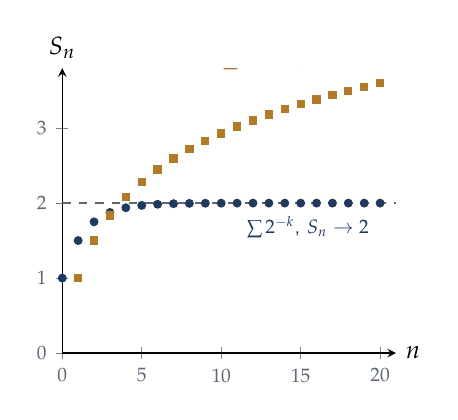
\begin{tikzpicture}
\begin{axis}[width=0.48\linewidth,height=5.2cm,axis lines=left,xmin=0,xmax=21,ymin=0,ymax=3.8,
  ticklabel style={font=\scriptsize\sffamily,color=Gris},xlabel={$n$},ylabel={$S_n$},
  every axis x label/.style={at={(ticklabel* cs:1)},anchor=west,font=\small},
  every axis y label/.style={at={(ticklabel* cs:1)},anchor=south,font=\small}]
\addplot[only marks,mark=*,mark size=1.4pt,Bleu,samples at={0,...,20}] {2-2^(-x)};
\addplot[only marks,mark=square*,mark size=1.3pt,Ocre] coordinates {(1,1)(2,1.5)(3,1.8333)(4,2.0833)(5,2.2833)(6,2.45)(7,2.5929)(8,2.7179)(9,2.829)(10,2.929)(11,3.0199)(12,3.1032)(13,3.1801)(14,3.2516)(15,3.3182)(16,3.3807)(17,3.4396)(18,3.4951)(19,3.5477)(20,3.5977)};
\addplot[asy,domain=0:21] {2};
\node[font=\scriptsize\sffamily,Bleu,anchor=north west] at (axis cs:11,1.95) {$\sum 2^{-k}$, $S_n\to2$};
\node[font=\scriptsize\sffamily,Ocre,anchor=south east] at (axis cs:20,3.65) {$\sum 1/k$, $S_n\to+\infty$};
\end{axis}
\end{tikzpicture}\hfill
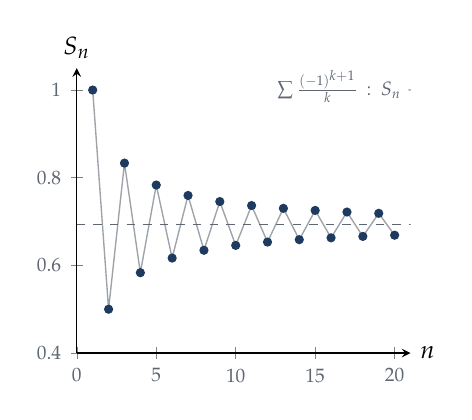
\begin{tikzpicture}
\begin{axis}[width=0.48\linewidth,height=5.2cm,axis lines=left,xmin=0,xmax=21,ymin=0.4,ymax=1.05,
  ticklabel style={font=\scriptsize\sffamily,color=Gris},xlabel={$n$},ylabel={$S_n$},
  every axis x label/.style={at={(ticklabel* cs:1)},anchor=west,font=\small},
  every axis y label/.style={at={(ticklabel* cs:1)},anchor=south,font=\small}]
\addplot[Gris!60,line width=0.5pt,mark=*,mark size=1.4pt,mark options={fill=Bleu,draw=Bleu}] coordinates {(1,1)(2,0.5)(3,0.8333)(4,0.5833)(5,0.7833)(6,0.6167)(7,0.7595)(8,0.6345)(9,0.7456)(10,0.6456)(11,0.7365)(12,0.6532)(13,0.7301)(14,0.6587)(15,0.7254)(16,0.6629)(17,0.7217)(18,0.6661)(19,0.7188)(20,0.6688)};
\addplot[asy,domain=0:21] {0.6931};
\node[font=\scriptsize\sffamily,Gris,anchor=south west] at (axis cs:12,0.95) {$\sum\frac{(-1)^{k+1}}k$ : $S_n\to\ln2$};
\end{axis}
\end{tikzpicture}
\caption{Sommes partielles. À gauche, deux séries à termes positifs : $(S_n)$ est croissante ; elle converge, ou tend vers $+\infty$.
À droite, une série alternée : $(S_n)$ oscille autour de sa limite en s'en rapprochant.}
\label{f:sommes}
\end{figure}

\begin{proposition}[linéarité, reste]\label{p:lin}
Si $\sum u_n$ et $\sum v_n$ convergent, alors $\sum(\lambda u_n+\mu v_n)$ converge et
$\sum_{n=0}^{+\infty}(\lambda u_n+\mu v_n)=\lambda\sum_{n=0}^{+\infty}u_n+\mu\sum_{n=0}^{+\infty}v_n$.
Si $\sum u_n$ converge, son reste tend vers $0$ : $R_n=S-S_n\to S-S=0$.
Si $\sum u_n$ converge et $\sum v_n$ diverge, alors $\sum(u_n+v_n)$ diverge (sinon $v_n=(u_n+v_n)-u_n$ donnerait une série convergente).
\end{proposition}

\begin{remarque}
La nature d'une série ne dépend pas de ses premiers termes : modifier un nombre fini de termes change la somme, pas la nature.
On peut donc commencer à $n=1$ ou $n=2$ quand le terme général n'est pas défini avant.
\end{remarque}

\subsubsection*{Une condition nécessaire}

\begin{theoreme}[divergence grossière]\label{t:grossiere}
Si $\sum u_n$ converge, alors $u_n\to0$. Par contraposée : si $(u_n)$ ne tend pas vers $0$, la série diverge ; on dit qu'elle
\emph{diverge grossièrement}.
\end{theoreme}

\begin{proof}
Si $S_n\to S$, alors $u_n=S_n-S_{n-1}\to S-S=0$.
\end{proof}

\begin{attention}
La réciproque est \emph{fausse} : $\frac1n\to0$, mais $\sum\frac1n$ diverge (proposition~\ref{p:harmonique}). « $u_n\to0$ » est le
premier test à faire, jamais une preuve de convergence.
\end{attention}

\begin{exemple}
$\sum1$, $\sum(-1)^n$, $\sum\cos n$, $\sum\left(1+\frac1n\right)^n$ divergent grossièrement. Pour $\cos n$ : si $\cos n\to0$,
alors $\cos(2n)=2\cos^2n-1\to-1$, ce qui contredit $\cos(2n)\to0$ (suite extraite).
\end{exemple}

\subsubsection*{Séries télescopiques}

\begin{theoreme}\label{t:telescopique}
La suite $(a_n)$ converge si et seulement si la série $\sum(a_{n+1}-a_n)$ converge. Dans ce cas
$\displaystyle\sum_{n=0}^{+\infty}(a_{n+1}-a_n)=\lim_{n\to+\infty}a_n-a_0$.
\end{theoreme}

\begin{proof}
Les termes se simplifient deux à deux : $\sum_{k=0}^{n-1}(a_{k+1}-a_k)=(a_1-a_0)+(a_2-a_1)+\dots+(a_n-a_{n-1})=a_n-a_0$. La
somme partielle converge si et seulement si $(a_n)$ converge.
\end{proof}

\begin{exemple}\label{x:tele}
$\frac1{n(n+1)}=\frac1n-\frac1{n+1}$, donc $\sum_{k=1}^n\frac1{k(k+1)}=1-\frac1{n+1}\to1$ : la série converge et
$\displaystyle\sum_{n=1}^{+\infty}\frac1{n(n+1)}=1$.
\end{exemple}

Le théorème sert dans les deux sens : pour calculer une somme (décomposer en éléments simples, faire apparaître une
différence), et pour \emph{étudier une suite} $(a_n)$ en étudiant la série $\sum(a_{n+1}-a_n)$ (exercice~\ref{e:s-gamma2}).

\subsubsection*{Séries géométriques et exponentielle}

\begin{theoreme}[séries géométriques]\label{t:geom}
Soit $q\in\C$. La série $\sum q^n$ converge si et seulement si $|q|<1$, et alors $\displaystyle\sum_{n=0}^{+\infty}q^n=\frac1{1-q}$.
\end{theoreme}

\begin{proof}
Si $|q|\geq1$, $|q^n|\geq1$ : divergence grossière. Si $|q|<1$, $S_n=\frac{1-q^{n+1}}{1-q}$ et $q^{n+1}\to0$, donc
$S_n\to\frac1{1-q}$.
\end{proof}

\begin{theoreme}[série exponentielle]\label{t:exp}
Pour tout $x\in\R$, la série $\sum\frac{x^n}{n!}$ converge et $\displaystyle\sum_{n=0}^{+\infty}\frac{x^n}{n!}=e^x$.
\end{theoreme}

\begin{proof}
L'inégalité de Taylor-Lagrange appliquée à $\exp$ entre $0$ et $x$ à l'ordre $n$ donne
$\left|e^x-\sum_{k=0}^n\frac{x^k}{k!}\right|\leq\frac{|x|^{n+1}}{(n+1)!}e^{|x|}$, qui tend vers $0$ par croissances comparées
($|x|^{n+1}=o((n+1)!)$, théorème~\ref{t:croiss}).
\end{proof}

\begin{methode}{Étudier une série « directement »}\label{m:directe}
\begin{enumerate}
\item Le terme général tend-il vers $0$ ? Sinon : divergence grossière, c'est fini.
\item Reconnaître une série de référence : géométrique, exponentielle, télescopique (décomposition en éléments simples,
$\ln\frac{n+1}n=\ln(n+1)-\ln n$, \dots).
\item Sinon, utiliser les théorèmes de comparaison des paragraphes suivants.
\end{enumerate}
\end{methode}

\serie{Exercices}

\begin{exo}{s-tele}{2}{télescopages}
\begin{enumerate}
\item Décomposer $\frac1{n(n+1)(n+2)}$ en éléments simples, puis calculer $\sum_{n=1}^{+\infty}\frac1{n(n+1)(n+2)}$.
\item Montrer que $\sum\ln\left(1+\frac1n\right)$ diverge.
\item Montrer que $\sum_{n\geq2}\ln\left(1-\frac1{n^2}\right)$ converge et calculer sa somme.
\end{enumerate}
\end{exo}

\begin{exo}{s-gamma2}{2}{une suite étudiée par une série}
On reprend $u_n=H_n-\ln n$ (exercice~\ref{e:s-gamma}). Donner un équivalent de $u_n-u_{n-1}$ ; en déduire, sans suites
adjacentes, que $(u_n)$ converge.
\end{exo}

% =====================================================================
\subsection{Séries à termes positifs}\label{ss:positifs}

Dans ce paragraphe, $u_n\geq0$ (au moins à partir d'un certain rang). Alors $S_{n+1}-S_n=u_{n+1}\geq0$ : la suite des sommes
partielles est \emph{croissante}, et tout repose sur le théorème de la limite monotone.

\begin{theoreme}\label{t:majoree}
Une série à termes positifs converge si et seulement si la suite de ses sommes partielles est majorée. Sinon, $S_n\to+\infty$.
\end{theoreme}

\begin{proof}
$(S_n)$ est croissante : elle converge si et seulement si elle est majorée (théorème~\ref{t:monotone}), et sinon elle tend vers
$+\infty$.
\end{proof}

\subsubsection*{Comparaison}

\begin{theoreme}[comparaison]\label{t:comparaison}
Si $0\leq u_n\leq v_n$ à partir d'un certain rang :
\begin{itemize}
\item si $\sum v_n$ converge, alors $\sum u_n$ converge (et $\sum_{n=0}^{+\infty}u_n\leq\sum_{n=0}^{+\infty}v_n$ si l'inégalité vaut pour tout $n$) ;
\item si $\sum u_n$ diverge, alors $\sum v_n$ diverge.
\end{itemize}
\end{theoreme}

\begin{proof}
Quitte à modifier les premiers termes (ce qui ne change pas la nature), $0\leq u_n\leq v_n$ pour tout $n$. Alors
$S_n=\sum_{k\leq n}u_k\leq T_n=\sum_{k\leq n}v_k$. Si $\sum v_n$ converge, $(T_n)$ est croissante de limite $T$, donc
$S_n\leq T_n\leq T$ : $(S_n)$ est majorée, la série $\sum u_n$ converge (théorème~\ref{t:majoree}) et $S\leq T$. La seconde
affirmation est la contraposée de la première.
\end{proof}

\begin{theoreme}[équivalents]\label{t:equivalents}
Si $u_n\sim v_n$ et $v_n\geq0$ à partir d'un certain rang, les séries $\sum u_n$ et $\sum v_n$ ont la même nature.
De même, si $u_n=O(v_n)$ ou $u_n=o(v_n)$ avec $u_n,v_n\geq0$, la convergence de $\sum v_n$ entraîne celle de $\sum u_n$.
\end{theoreme}

\begin{proof}
Si $\frac{u_n}{v_n}\to1$, il existe un rang à partir duquel $\frac12\leq\frac{u_n}{v_n}\leq\frac32$, c'est-à-dire
$0\leq\frac12v_n\leq u_n\leq\frac32v_n$. Le théorème de comparaison, appliqué deux fois, donne le résultat. Si $u_n=O(v_n)$,
$0\leq u_n\leq Mv_n$ pour une constante $M$, et $\sum Mv_n$ converge si $\sum v_n$ converge.
\end{proof}

\begin{attention}
L'hypothèse de \emph{signe} est indispensable. $u_n=\frac{(-1)^n}{\sqrt n}+\frac1n$ et $v_n=\frac{(-1)^n}{\sqrt n}$ sont
équivalentes, mais $\sum v_n$ converge et $\sum u_n$ diverge (§\ref{ss:absolue}). Toujours écrire : « $u_n\sim v_n$, \textbf{avec
$v_n\geq0$} ».
\end{attention}

\subsubsection*{Comparaison avec une intégrale}

On utilisera la définition suivante, développée dans le chapitre sur les intégrales généralisées.

\begin{definition}
Soit $f$ continue sur $[a,+\infty[$. Si $\int_a^Xf(t)\,dt$ a une limite finie quand $X\to+\infty$, on dit que l'intégrale
$\int_a^{+\infty}f(t)\,dt$ \emph{converge}, et on note $\int_a^{+\infty}f(t)\,dt$ cette limite. Sinon elle \emph{diverge}.
\end{definition}

\begin{figure}[h]
\centering
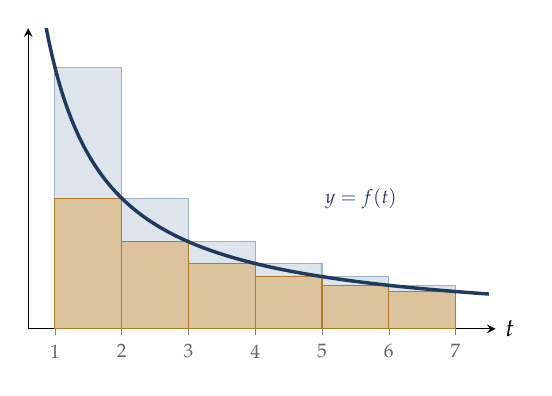
\begin{tikzpicture}
\begin{axis}[width=0.62\linewidth,height=5.4cm,axis lines=left,xmin=0.6,xmax=7.6,ymin=0,ymax=1.15,
  ticklabel style={font=\scriptsize\sffamily,color=Gris},xtick={1,...,7},ytick=\empty,
  xlabel={$t$},every axis x label/.style={at={(ticklabel* cs:1)},anchor=west,font=\small}]
\addplot[fill=BleuClair!35,draw=BleuClair] coordinates {(1,0) (1,1.0000) (2,1.0000) (2,0)} \closedcycle;
\addplot[fill=BleuClair!35,draw=BleuClair] coordinates {(2,0) (2,0.5000) (3,0.5000) (3,0)} \closedcycle;
\addplot[fill=BleuClair!35,draw=BleuClair] coordinates {(3,0) (3,0.3333) (4,0.3333) (4,0)} \closedcycle;
\addplot[fill=BleuClair!35,draw=BleuClair] coordinates {(4,0) (4,0.2500) (5,0.2500) (5,0)} \closedcycle;
\addplot[fill=BleuClair!35,draw=BleuClair] coordinates {(5,0) (5,0.2000) (6,0.2000) (6,0)} \closedcycle;
\addplot[fill=BleuClair!35,draw=BleuClair] coordinates {(6,0) (6,0.1667) (7,0.1667) (7,0)} \closedcycle;
\addplot[fill=Ocre!45,draw=Ocre] coordinates {(1,0) (1,0.5000) (2,0.5000) (2,0)} \closedcycle;
\addplot[fill=Ocre!45,draw=Ocre] coordinates {(2,0) (2,0.3333) (3,0.3333) (3,0)} \closedcycle;
\addplot[fill=Ocre!45,draw=Ocre] coordinates {(3,0) (3,0.2500) (4,0.2500) (4,0)} \closedcycle;
\addplot[fill=Ocre!45,draw=Ocre] coordinates {(4,0) (4,0.2000) (5,0.2000) (5,0)} \closedcycle;
\addplot[fill=Ocre!45,draw=Ocre] coordinates {(5,0) (5,0.1667) (6,0.1667) (6,0)} \closedcycle;
\addplot[fill=Ocre!45,draw=Ocre] coordinates {(6,0) (6,0.1429) (7,0.1429) (7,0)} \closedcycle;
\addplot[arcetude,domain=0.85:7.5,samples=120] {1/x};
\node[font=\scriptsize\sffamily,Bleu,anchor=south west] at (axis cs:4.9,0.42) {$y=f(t)$};
\end{axis}
\end{tikzpicture}
\caption{$f$ décroissante. Sur $[k,k+1]$, le rectangle orange (hauteur $f(k+1)$) est sous la courbe, le rectangle bleu (hauteur
$f(k)$) au-dessus : $f(k+1)\leq\int_k^{k+1}f\leq f(k)$.}
\label{f:serieint}
\end{figure}

\begin{theoreme}[comparaison série-intégrale]\label{t:serieint}
Soit $f$ continue, positive et décroissante sur $[n_0,+\infty[$. Alors, pour $n>n_0$,
\[\sum_{k=n_0+1}^nf(k)\ \leq\ \int_{n_0}^nf(t)\,dt\ \leq\ \sum_{k=n_0}^{n-1}f(k),\]
et la série $\sum f(n)$ et l'intégrale $\int_{n_0}^{+\infty}f(t)\,dt$ ont la même nature.
\end{theoreme}

\begin{proof}
\etape{Encadrement}Pour $k\geq n_0$ et $t\in[k,k+1]$, la décroissance donne $f(k+1)\leq f(t)\leq f(k)$. On intègre sur
$[k,k+1]$ (intervalle de longueur $1$) : $f(k+1)\leq\int_k^{k+1}f\leq f(k)$ (figure~\ref{f:serieint}). On somme pour $k$ de $n_0$ à
$n-1$ et on utilise la relation de Chasles : c'est l'encadrement annoncé.

\etape{Si l'intégrale converge}La fonction $X\mapsto\int_{n_0}^Xf$ est croissante ($f\geq0$) et a une limite $I$, donc
$\int_{n_0}^nf\leq I$. L'encadrement donne $\sum_{k=n_0+1}^nf(k)\leq I$ : les sommes partielles de la série à termes positifs
$\sum f(n)$ sont majorées, elle converge.

\etape{Si la série converge}Soit $S$ sa somme. Pour $X\geq n_0$, en prenant un entier $n\geq X$ :
$\int_{n_0}^Xf\leq\int_{n_0}^nf\leq\sum_{k=n_0}^{n-1}f(k)\leq S$. La fonction croissante $X\mapsto\int_{n_0}^Xf$ est majorée :
elle a une limite finie, l'intégrale converge.
\end{proof}

\begin{theoreme}[séries de Riemann]\label{t:riemann}
Soit $\alpha\in\R$. L'intégrale $\int_1^{+\infty}\frac{dt}{t^\alpha}$ et la série $\sum_{n\geq1}\frac1{n^\alpha}$ convergent si et
seulement si $\alpha>1$.
\end{theoreme}

\begin{proof}
\etape{Intégrale}Pour $\alpha=1$, $\int_1^X\frac{dt}t=\ln X\to+\infty$. Pour $\alpha\neq1$,
$\int_1^X\frac{dt}{t^\alpha}=\frac1{1-\alpha}\left(X^{1-\alpha}-1\right)$, qui tend vers $\frac1{\alpha-1}$ si $\alpha>1$ et vers
$+\infty$ si $\alpha<1$.

\etape{Série}Si $\alpha\leq0$, $\frac1{n^\alpha}\not\to0$ : divergence grossière. Si $\alpha>0$, $t\mapsto\frac1{t^\alpha}$ est
continue, positive et décroissante sur $[1,+\infty[$ : la série a la nature de l'intégrale.
\end{proof}

\begin{proposition}[série harmonique]\label{p:harmonique}
$H_n=\sum_{k=1}^n\frac1k$ vérifie $\ln(n+1)\leq H_n\leq1+\ln n$. En particulier $H_n\to+\infty$ et $H_n\sim\ln n$.
\end{proposition}

\begin{proof}
Théorème~\ref{t:serieint} avec $f(t)=\frac1t$ et $n_0=1$ : $H_n-1\leq\int_1^n\frac{dt}t=\ln n$, et
$\ln(n+1)=\int_1^{n+1}\frac{dt}t\leq H_n$. On divise par $\ln n$ : $\frac{\ln(n+1)}{\ln n}\to1$ et $\frac{1+\ln n}{\ln n}\to1$.
\end{proof}

\begin{enpratique}
La même méthode \emph{encadre un reste}. Pour $\sum\frac1{k^2}$ : $\int_{k}^{k+1}\frac{dt}{t^2}\leq\frac1{k^2}\leq\int_{k-1}^{k}\frac{dt}{t^2}$
($k\geq2$) ; on somme de $n+1$ à $N$ et on fait $N\to+\infty$ :
\[\frac1{n+1}\leq R_n=\sum_{k=n+1}^{+\infty}\frac1{k^2}\leq\frac1n,\qquad\text{donc}\qquad R_n\sim\frac1n.\]
Pour obtenir $S=\sum_{n\geq1}\frac1{n^2}$ à $10^{-4}$ près, il suffit de $\frac1n\leq10^{-4}$ : $n=10^4$ termes ($S=\frac{\pi^2}6$,
résultat admis). Pour $\sum\frac1{k^\alpha}$, $\alpha>1$, on obtient de même $R_n\sim\frac1{(\alpha-1)n^{\alpha-1}}$
(exercice~\ref{e:s-reste}).
\end{enpratique}

\subsubsection*{Règle de d'Alembert}

\begin{theoreme}[règle de d'Alembert]\label{t:dalembert}
Soit $\sum u_n$ une série à termes \emph{strictement} positifs telle que $\frac{u_{n+1}}{u_n}\to\ell\in[0,+\infty]$.
\begin{itemize}
\item Si $\ell<1$, la série converge.
\item Si $\ell>1$, la série diverge (grossièrement).
\item Si $\ell=1$, on ne peut pas conclure.
\end{itemize}
\end{theoreme}

\begin{proof}
\etape{$\ell<1$}On fixe $q=\frac{1+\ell}2$, de sorte que $\ell<q<1$. Comme $\frac{u_{n+1}}{u_n}\to\ell<q$, il existe $N$ tel que
$\frac{u_{k+1}}{u_k}\leq q$ pour $k\geq N$. En multipliant ces inégalités de $k=N$ à $n-1$ (produit télescopique) :
$u_n\leq u_Nq^{n-N}=Kq^n$ avec $K=u_Nq^{-N}$. La série géométrique $\sum q^n$ converge ($0<q<1$) : par comparaison, $\sum u_n$
converge.

\etape{$\ell>1$}À partir d'un rang $N$, $\frac{u_{n+1}}{u_n}>1$ : la suite $(u_n)_{n\geq N}$ est croissante et strictement positive,
elle ne tend pas vers $0$.

\etape{$\ell=1$}$u_n=\frac1n$ et $u_n=\frac1{n^2}$ donnent tous deux $\ell=1$ ; la première série diverge, la seconde converge.
\end{proof}

\begin{enpratique}
D'Alembert est fait pour les termes contenant des \emph{factorielles} ou des \emph{puissances $n$-ièmes} ($a^n$, $n^n$) : le quotient
se simplifie. Pour les fractions rationnelles en $n$, on trouve toujours $\ell=1$ : utiliser plutôt un équivalent et Riemann.
\end{enpratique}

\begin{exemple}
$u_n=\frac{n^2}{2^n}$ : $\frac{u_{n+1}}{u_n}=\frac12\left(\frac{n+1}n\right)^2\to\frac12<1$, la série converge.
$u_n=\frac{n!}{n^n}$ : $\frac{u_{n+1}}{u_n}=\frac{(n+1)\,n^n}{(n+1)^{n+1}}=\left(1+\frac1n\right)^{-n}\to\frac1e<1$, la série
converge ; en particulier $n!=o(n^n)$.
\end{exemple}

\begin{methode}{Série à termes positifs : quel outil ?}\label{m:positifs}
\begin{enumerate}
\item Chercher un \emph{équivalent} simple $v_n\geq0$ du terme général (développements limités, termes dominants).
\item Comparer à une série de Riemann $\sum\frac1{n^\alpha}$ ou géométrique. Pour montrer la convergence, il suffit souvent de
prouver $n^\alpha u_n\to0$ avec $\alpha>1$ (alors $u_n=o(\frac1{n^\alpha})$) ; pour la divergence, $nu_n\to+\infty$ (alors
$u_n\geq\frac1n$ à partir d'un rang).
\item Factorielles, puissances $n$-ièmes : d'Alembert.
\item $u_n=f(n)$ avec $f$ décroissante d'intégrale calculable (par exemple $\frac1{n\ln n}$) : comparaison série-intégrale.
\end{enumerate}
\end{methode}

\begin{exemple}
$\sum\frac{\ln n}{n^2}$ : $n^{3/2}\cdot\frac{\ln n}{n^2}=\frac{\ln n}{\sqrt n}\to0$, donc $\frac{\ln n}{n^2}=o\left(\frac1{n^{3/2}}\right)$ et la
série converge ($\frac32>1$). $\sum\frac1{\sqrt n\ln n}$ : $n\cdot\frac1{\sqrt n\ln n}=\frac{\sqrt n}{\ln n}\to+\infty$, donc
$\frac1{\sqrt n\ln n}\geq\frac1n$ à partir d'un rang, et la série diverge. $\sum\frac1{n\ln n}$ : $t\mapsto\frac1{t\ln t}$ est
décroissante sur $[2,+\infty[$ et $\int_2^X\frac{dt}{t\ln t}=\ln(\ln X)-\ln(\ln2)\to+\infty$ : la série diverge.
\end{exemple}

\serie{Exercices}

\begin{exo}{s-nature}{2}{nature de séries à termes positifs}
Déterminer la nature des séries de terme général :
\[\text{(a)}\ \frac{n^2+1}{n^4+3}\qquad\text{(b)}\ \frac1{\sqrt{n(n+1)}}\qquad\text{(c)}\ 1-\cos\frac1n\qquad\text{(d)}\ \frac1{\ln n+e^n}\qquad\text{(e)}\ n^2e^{-\sqrt n}\qquad\text{(f)}\ \frac{\ln n}n.\]
\end{exo}

\begin{exo}{s-dal}{2}{règle de d'Alembert}
\begin{enumerate}
\item Soit $a>0$. Montrer que $\sum\frac{a^n}{n!}$ converge ; en déduire que $a^n=o(n!)$.
\item Nature de $\sum\frac{(2n)!}{(n!)^2\,4^n}$ ? Pourquoi d'Alembert ne permet-il pas de conclure ? (On admettra que
$\frac{(2n)!}{(n!)^24^n}\sim\frac1{\sqrt{\pi n}}$.)
\end{enumerate}
\end{exo}

\begin{exo}{s-reste}{3}{équivalent d'un reste}
Soit $\alpha>1$. Montrer, par comparaison avec une intégrale, que $\displaystyle\sum_{k=n+1}^{+\infty}\frac1{k^\alpha}\sim\frac1{(\alpha-1)n^{\alpha-1}}$.
\end{exo}

% =====================================================================
\subsection{Convergence absolue, séries alternées}\label{ss:absolue}

On revient à des séries de signe quelconque, réelles ou complexes. Les théorèmes du §\ref{ss:positifs} ne s'appliquent pas
directement ; l'idée est de s'y ramener en passant au module.

\begin{definition}
La série $\sum u_n$ est \emph{absolument convergente} si la série à termes positifs $\sum|u_n|$ converge.
\end{definition}

\begin{theoreme}\label{t:acv}
Une série absolument convergente est convergente, et $\displaystyle\left|\sum_{n=0}^{+\infty}u_n\right|\leq\sum_{n=0}^{+\infty}|u_n|$.
\end{theoreme}

\begin{proof}
\etape{Cas réel}On écrit $u_n=u_n^+-u_n^-$, avec $u_n^+=\max(u_n,0)$ et $u_n^-=\max(-u_n,0)$. Ces deux suites sont positives
et majorées par $|u_n|$ : par comparaison, $\sum u_n^+$ et $\sum u_n^-$ convergent, donc leur différence $\sum u_n$ aussi
(proposition~\ref{p:lin}).

\etape{Cas complexe}$|\mathrm{Re}\,u_n|\leq|u_n|$ et $|\mathrm{Im}\,u_n|\leq|u_n|$ : les séries réelles $\sum\mathrm{Re}\,u_n$ et
$\sum\mathrm{Im}\,u_n$ sont absolument convergentes, donc convergentes (cas réel), et $\sum u_n=\sum(\mathrm{Re}\,u_n+i\,\mathrm{Im}\,u_n)$
converge.

\etape{Inégalité}Pour tout $N$, $\left|\sum_{n=0}^Nu_n\right|\leq\sum_{n=0}^N|u_n|\leq\sum_{n=0}^{+\infty}|u_n|$ ; on fait $N\to+\infty$.
\end{proof}

\begin{theoreme}\label{t:acvcomp}
Soient $\sum u_n$ une série complexe et $\sum v_n$ une série à termes positifs \emph{convergente}. Si $u_n=O(v_n)$ (en
particulier si $u_n=o(v_n)$), alors $\sum u_n$ est absolument convergente. Notamment, si $u_n=O\left(\frac1{n^\alpha}\right)$ avec
$\alpha>1$, $\sum u_n$ converge absolument.
\end{theoreme}

\begin{proof}
$|u_n|\leq Mv_n$ à partir d'un rang, et $\sum Mv_n$ converge : on conclut par comparaison des séries à termes positifs.
\end{proof}

\begin{exemple}
$\sum\frac{(-1)^n}{n^2}$, $\sum\frac{\cos n}{n^2}$, $\sum\frac{e^{in\theta}}{n^{3/2}}$ convergent absolument : leur module est majoré par
le terme d'une série de Riemann convergente. Pour $z\in\C$, $\sum\frac{z^n}{n^2}$ converge absolument si $|z|\leq1$, et diverge
grossièrement si $|z|>1$ (croissances comparées).
\end{exemple}

\subsubsection*{Séries alternées}

Une série convergente n'est pas toujours absolument convergente : on dit alors qu'elle est \emph{semi-convergente}. Les
exemples les plus simples sont fournis par le théorème suivant.

\begin{theoreme}[critère des séries alternées]\label{t:alternees}
Soit $(a_n)$ une suite réelle \emph{positive, décroissante, de limite nulle}. Alors la série $\sum(-1)^na_n$ converge. De plus,
sa somme $S$ est comprise entre deux sommes partielles consécutives, et le reste vérifie
\[|R_n|=\left|\sum_{k=n+1}^{+\infty}(-1)^ka_k\right|\leq a_{n+1},\]
et $R_n$ a le signe de son premier terme $(-1)^{n+1}a_{n+1}$.
\end{theoreme}

\begin{proof}
\etape{Les sommes paires décroissent}$S_{2n+2}-S_{2n}=a_{2n+2}-a_{2n+1}\leq0$.
\etape{Les sommes impaires croissent}$S_{2n+3}-S_{2n+1}=-a_{2n+3}+a_{2n+2}\geq0$.
\etape{Leur écart tend vers $0$}$S_{2n+1}-S_{2n}=-a_{2n+1}\to0$.

Les suites $(S_{2n+1})$ et $(S_{2n})$ sont adjacentes (théorème~\ref{t:adjacentes}) : elles convergent vers une même limite $S$,
avec $S_{2n+1}\leq S\leq S_{2n}$. Les deux suites extraites paire et impaire ayant la même limite, $(S_n)$ converge vers $S$.

\etape{Reste}$S$ est entre $S_n$ et $S_{n+1}$ (l'une est paire, l'autre impaire), donc $|R_n|=|S-S_n|\leq|S_{n+1}-S_n|=a_{n+1}$.
Le signe découle de la même position.
\end{proof}

\begin{exemple}
$\sum\frac{(-1)^n}n$, $\sum\frac{(-1)^n}{\sqrt n}$, $\sum(-1)^n\sin\frac1n$ convergent par le critère (pour la dernière,
$\sin\frac1n$ est positive et décroissante car $\sin$ croît sur $[0,1]$). Elles ne convergent pas absolument : $\frac1n$,
$\frac1{\sqrt n}$, $\sin\frac1n\sim\frac1n$ sont des termes de séries divergentes. Ce sont des séries semi-convergentes. On
montre (exercice~\ref{e:s-alt}) que $\sum_{n=1}^{+\infty}\frac{(-1)^{n+1}}n=\ln2$ (figure~\ref{f:sommes}).
\end{exemple}

\begin{attention}
\begin{itemize}[leftmargin=1.1em]
\item Les trois hypothèses comptent, la \emph{décroissance} en particulier, et elle se vérifie (dérivée, ou quotient).
\item Pour une série de signe quelconque, on \emph{n'utilise pas} d'équivalent : $\frac{(-1)^n}{\sqrt n+(-1)^n}\sim\frac{(-1)^n}{\sqrt n}$,
mais la première série diverge et la seconde converge (méthode~\ref{m:asympt}).
\item Si la série converge absolument, inutile de recourir au critère : $\sum\frac{(-1)^n}{n^2}$ se traite par la convergence absolue.
\end{itemize}
\end{attention}

\begin{methode}{Série de signe quelconque : développement asymptotique}\label{m:asympt}
Quand ni la convergence absolue ni le critère des séries alternées ne s'appliquent directement :
\begin{enumerate}
\item développer $u_n$ jusqu'à obtenir un reste $O\left(\frac1{n^\alpha}\right)$ avec $\alpha>1$ ;
\item écrire $u_n=a_n+b_n+\dots+O\left(\frac1{n^\alpha}\right)$ où chaque terme est d'un type connu (alterné, de signe constant) ;
\item conclure par linéarité : somme de séries convergentes, ou convergente $+$ divergente.
\end{enumerate}
\end{methode}

\begin{exemple}
$u_n=\frac{(-1)^n}{\sqrt n+(-1)^n}=\frac{(-1)^n}{\sqrt n}\cdot\frac1{1+\frac{(-1)^n}{\sqrt n}}
=\frac{(-1)^n}{\sqrt n}\left(1-\frac{(-1)^n}{\sqrt n}+O\left(\frac1n\right)\right)=\frac{(-1)^n}{\sqrt n}-\frac1n+O\left(\frac1{n^{3/2}}\right)$.
$\sum\frac{(-1)^n}{\sqrt n}$ converge (critère), $\sum O\left(\frac1{n^{3/2}}\right)$ converge absolument, $\sum\frac1n$ diverge : la série
$\sum u_n$ \emph{diverge}.
\end{exemple}

\serie{Exercices}

\begin{exo}{s-alt}{2}{séries alternées}
\begin{enumerate}
\item Montrer que $\sum_{n\geq1}\frac{(-1)^{n+1}}n$ converge. En intégrant $\sum_{k=0}^{n-1}(-t)^k=\frac{1-(-t)^n}{1+t}$ sur $[0,1]$,
montrer que sa somme vaut $\ln2$.
\item Combien de termes faut-il sommer pour approcher $\ln 2$ à $10^{-3}$ près par cette série ?
\end{enumerate}
\end{exo}

\begin{exo}{s-asympt}{3}{développement asymptotique}
Déterminer la nature des séries de terme général
\[\text{(a)}\ \ln\left(1+\frac{(-1)^n}{\sqrt n}\right)\ (n\geq2)\qquad\text{(b)}\ \frac{(-1)^n}{n+(-1)^n}\ (n\geq2)\qquad\text{(c)}\ \frac{(-1)^n}{n^\alpha}\ (\alpha\in\R).\]
\end{exo}

% =====================================================================
\subsection{Produit de Cauchy}\label{ss:cauchy}

On sait additionner deux séries convergentes terme à terme. Les multiplier est plus délicat : en général
$\sum u_n\cdot\sum v_n\neq\sum u_nv_n$ (déjà $(u_0+u_1)(v_0+v_1)\neq u_0v_0+u_1v_1$). Pour développer le produit, on regroupe les
termes $u_pv_q$ selon la valeur de $p+q$.

\begin{definition}
Le \emph{produit de Cauchy} des séries $\sum u_n$ et $\sum v_n$ est la série $\sum w_n$, où
$\displaystyle w_n=\sum_{p=0}^nu_pv_{n-p}=u_0v_n+u_1v_{n-1}+\dots+u_nv_0$.
\end{definition}

\begin{figure}[h]
\centering
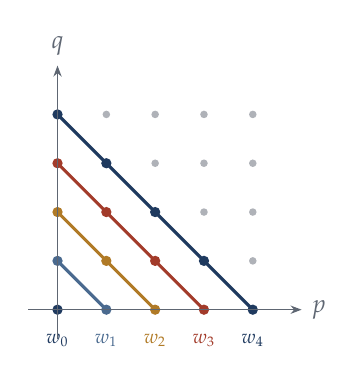
\begin{tikzpicture}[scale=0.62]
\foreach \p in {0,...,4} \foreach \q in {0,...,4} {\fill[Gris!50] (\p,\q) circle (2.2pt);}
\foreach \n/\c in {0/Bleu,1/BleuMoyen,2/Ocre,3/Brique,4/Bleu} {
  \draw[\c,line width=1.1pt] (\n,0) -- (0,\n);
  \foreach \p in {0,...,\n} {\pgfmathtruncatemacro{\q}{\n-\p}\fill[\c] (\p,\q) circle (3pt);}
  \node[font=\scriptsize\sffamily,\c,anchor=north] at (\n,-0.3) {$w_{\n}$};
}
\draw[Gris,-{Stealth[length=4pt]}] (-0.6,0) -- (5,0) node[right,font=\small] {$p$};
\draw[Gris,-{Stealth[length=4pt]}] (0,-0.6) -- (0,5) node[above,font=\small] {$q$};
\end{tikzpicture}
\caption{Le terme $u_pv_q$ est placé au point $(p,q)$. $w_n$ regroupe les termes d'une même diagonale $p+q=n$.}
\end{figure}

\begin{theoreme}[admis]\label{t:cauchy}
Si $\sum u_n$ et $\sum v_n$ sont absolument convergentes, leur produit de Cauchy $\sum w_n$ est absolument convergent et
\[\sum_{n=0}^{+\infty}w_n=\left(\sum_{n=0}^{+\infty}u_n\right)\left(\sum_{n=0}^{+\infty}v_n\right).\]
\end{theoreme}

\begin{exemple}
Pour $|x|<1$, $\sum x^n$ converge absolument. Son produit de Cauchy avec elle-même a pour terme $w_n=\sum_{p=0}^nx^px^{n-p}=(n+1)x^n$.
Donc $\displaystyle\sum_{n=0}^{+\infty}(n+1)x^n=\frac1{(1-x)^2}$.
\end{exemple}

\begin{proposition}[exponentielle complexe]\label{p:expc}
Pour $z\in\C$, la série $\sum\frac{z^n}{n!}$ converge absolument ; on note $\exp(z)$ sa somme. Pour tous $a,b\in\C$,
$\exp(a+b)=\exp(a)\exp(b)$.
\end{proposition}

\begin{proof}
Si $z\neq0$, $\frac{|z|^{n+1}/(n+1)!}{|z|^n/n!}=\frac{|z|}{n+1}\to0$ : d'Alembert donne la convergence absolue. Le produit de Cauchy
de $\sum\frac{a^n}{n!}$ et $\sum\frac{b^n}{n!}$ a pour terme, par la formule du binôme,
$w_n=\sum_{p=0}^n\frac{a^p}{p!}\frac{b^{n-p}}{(n-p)!}=\frac1{n!}\sum_{p=0}^n\binom npa^pb^{n-p}=\frac{(a+b)^n}{n!}$. Le théorème~\ref{t:cauchy}
donne $\exp(a)\exp(b)=\sum\frac{(a+b)^n}{n!}=\exp(a+b)$.
\end{proof}

\serie{Exercice}

\begin{exo}{s-cauchy}{2}{produit de Cauchy}
\begin{enumerate}
\item Calculer $\left(\sum_{n=0}^{+\infty}\frac1{2^n}\right)^2$ et $\sum_{n=0}^{+\infty}\frac1{4^n}$ : que constate-t-on ?
\item Pour $|x|<1$, calculer $\sum_{n=0}^{+\infty}nx^n$, puis $\sum_{n=0}^{+\infty}\frac{n}{2^n}$.
\end{enumerate}
\end{exo}

% =====================================================================
\subsection{Quelle méthode ? Synthèse}\label{ss:synthese}

\begin{figure}[h]
\centering
\begin{tikzpicture}[
  q/.style={draw=Bleu,fill=Fond,rounded corners=3pt,font=\small\sffamily,align=center,inner sep=5pt,text width=3.6cm},
  r/.style={draw=Ocre,fill=Ocre!8,rounded corners=3pt,font=\small\sffamily,align=center,inner sep=5pt,text width=3.4cm},
  f/.style={-{Stealth[length=5pt]},Gris,line width=0.7pt},
  l/.style={font=\scriptsize\sffamily,Gris}]
\node[q] (a) at (0,0) {$u_n\to0$ ?};
\node[r] (gr) at (5,0) {divergence grossière};
\node[q] (b) at (0,-1.9) {signe constant ?};
\node[r] (pos) at (5,-1.9) {équivalent, Riemann, d'Alembert, intégrale (§\ref{ss:positifs})};
\node[q] (c) at (0,-3.8) {$\sum|u_n|$ converge ?};
\node[r] (acv) at (5,-3.8) {convergence absolue, donc convergence};
\node[q] (d) at (0,-5.7) {$(-1)^na_n$, $a_n\downarrow0$ ?};
\node[r] (alt) at (5,-5.7) {critère des séries alternées};
\node[r] (dev) at (0,-7.6) {développement asymptotique (méthode~\ref{m:asympt})};
\draw[f] (a) -- node[l,above]{non} (gr);
\draw[f] (a) -- node[l,right]{oui} (b);
\draw[f] (b) -- node[l,above]{oui} (pos);
\draw[f] (b) -- node[l,right]{non} (c);
\draw[f] (c) -- node[l,above]{oui} (acv);
\draw[f] (c) -- node[l,right]{non} (d);
\draw[f] (d) -- node[l,above]{oui} (alt);
\draw[f] (d) -- node[l,right]{non} (dev);
\end{tikzpicture}
\caption{Étudier la nature de $\sum u_n$ : l'ordre des questions.}
\label{f:arbre}
\end{figure}

\begin{center}
\renewcommand{\arraystretch}{1.35}
\small
\begin{tabular}{p{0.36\linewidth}p{0.57\linewidth}}
\hline
\textbf{Le terme général contient\dots} & \textbf{Outil}\\\hline
une fraction rationnelle en $n$, des racines & équivalent $\frac C{n^\alpha}$, Riemann\\
$\ln$, $\exp$, $\sin$, $\cos$ de quantités qui tendent vers $0$ & développement limité, puis équivalent\\
$\ln n$ et des puissances & $n^\alpha u_n\to0$ ($\alpha>1$) ou $nu_n\to+\infty$\\
$n!$, $a^n$, $n^n$ & d'Alembert, croissances comparées\\
$f(n)$, $f$ décroissante, intégrable explicitement & comparaison série-intégrale\\
$(-1)^n$ & convergence absolue, sinon critère des séries alternées, sinon développement\\
une différence $a_{n+1}-a_n$ & série télescopique\\\hline
\end{tabular}
\end{center}

\begin{attention}\textbf{Pièges fréquents.}
\begin{itemize}[leftmargin=1.1em]
\item Conclure à la convergence parce que $u_n\to0$.
\item Utiliser un équivalent pour une série qui n'est pas de signe constant.
\item Appliquer d'Alembert quand la limite vaut $1$, ou à une fraction rationnelle.
\item Écrire $\sum_{n=0}^{+\infty}u_n$ avant d'avoir prouvé la convergence ; oublier la décroissance dans le critère des séries alternées.
\item Confondre l'intégrale $\int_1^{+\infty}\frac{dt}{t^\alpha}$ (convergente pour $\alpha>1$) et $\int_0^1\frac{dt}{t^\alpha}$ (convergente pour $\alpha<1$).
\end{itemize}
\end{attention}

\begin{essentiel}
\begin{itemize}[leftmargin=1.1em,itemsep=2pt]
\item $\sum u_n$ converge $\Rightarrow u_n\to0$ ; la réciproque est fausse ($\sum\frac1n$).
\item Références : $\sum q^n$ ($|q|<1$), $\sum\frac1{n^\alpha}$ ($\alpha>1$), $\sum\frac{x^n}{n!}=e^x$, télescopiques.
\item Termes positifs : comparaison, équivalents, d'Alembert, comparaison série-intégrale (qui encadre aussi les sommes et les restes).
\item Signe quelconque : convergence absolue $\Rightarrow$ convergence ; séries alternées ; développement asymptotique.
\item Produit de Cauchy de deux séries absolument convergentes : la somme est le produit des sommes.
\end{itemize}
\end{essentiel}

% =====================================================================
%                              CORRIGÉS
% =====================================================================
\clearpage
\renewcommand{\ongletcouleur}{Ocre}
\section{Corrigés}\label{sec:corriges-series}

\begin{corrige}{s-equiv}
$\left(1+\frac1n\right)^n=e^{x_n}$ avec $x_n=n\ln\left(1+\frac1n\right)=n\left(\frac1n-\frac1{2n^2}+o\left(\frac1{n^2}\right)\right)=1-\frac1{2n}+o\left(\frac1n\right)$.
Donc $x_n\to1$ et, par continuité de $\exp$, $\left(1+\frac1n\right)^n\to e$. Ensuite
$\left(1+\frac1n\right)^n-e=e\left(e^{x_n-1}-1\right)$ avec $x_n-1\to0$, et $e^y-1\sim y$ quand $y\to0$ :
$\left(1+\frac1n\right)^n-e\sim e(x_n-1)\sim-\frac e{2n}$.
\piege{écrire $\left(1+\frac1n\right)^n\sim e^{1}$ « car $n\ln(1+\frac1n)\sim1$ » donne la limite, mais rien sur l'écart : on ne
compose pas les équivalents par $\exp$. Il faut le développement de $x_n-1$.}
\end{corrige}

\begin{corrige}{s-gamma}
$v_{n+1}-v_n=\frac1{n}-\ln\left(1+\frac1n\right)\geq0$ (avec $\ln(1+x)\leq x$). Et
$u_{n+1}-u_n=\frac1{n+1}-\ln\frac{n+1}n=\frac1{n+1}+\ln\left(1-\frac1{n+1}\right)\leq\frac1{n+1}-\frac1{n+1}=0$. Enfin
$u_n-v_n=\frac1n\to0$ : les suites sont adjacentes et convergent vers $\gamma$. Comme $(v_n)$ croît, $\gamma\geq v_2=1+\frac12-\ln2-\frac12=1-\ln2>0$.
Enfin $u_n-\gamma\to0$ s'écrit $H_n=\ln n+\gamma+o(1)$. (Numériquement $\gamma\approx0{,}5772$.)
\end{corrige}

\begin{corrige}{s-tele}
\q{1.} $\frac1{n(n+1)(n+2)}=\frac1{2n}-\frac1{n+1}+\frac1{2(n+2)}=\frac12\left(\frac1{n(n+1)}-\frac1{(n+1)(n+2)}\right)$. C'est
$a_n-a_{n+1}$ avec $a_n=\frac1{2n(n+1)}\to0$, donc la série converge et $\sum_{n=1}^{+\infty}\frac1{n(n+1)(n+2)}=a_1-0=\frac14$.

\q{2.} $\ln\left(1+\frac1n\right)=\ln(n+1)-\ln n$ : $S_n=\sum_{k=1}^n\ln\left(1+\frac1k\right)=\ln(n+1)\to+\infty$, la série diverge.
Comme $\ln\left(1+\frac1n\right)\sim\frac1n\geq0$, on retrouve au passage la divergence de $\sum\frac1n$.

\q{3.} $\ln\left(1-\frac1{n^2}\right)=\ln\frac{(n-1)(n+1)}{n^2}=\big(\ln(n+1)-\ln n\big)-\big(\ln n-\ln(n-1)\big)$. Donc
$\sum_{k=2}^n\ln\left(1-\frac1{k^2}\right)=\big(\ln(n+1)-\ln2\big)-\big(\ln n-\ln1\big)=\ln\frac{n+1}n-\ln2\to-\ln2$. La série converge, de
somme $-\ln2$.
\end{corrige}

\begin{corrige}{s-gamma2}
Pour $n\geq2$, $u_n-u_{n-1}=\frac1n+\ln\left(1-\frac1n\right)=\frac1n-\frac1n-\frac1{2n^2}+o\left(\frac1{n^2}\right)\sim-\frac1{2n^2}$.
Le terme $u_{n-1}-u_n\sim\frac1{2n^2}$ est positif à partir d'un rang, et $\sum\frac1{n^2}$ converge : la série $\sum(u_n-u_{n-1})$
converge, donc la suite $(u_n)$ converge (théorème~\ref{t:telescopique}).
\end{corrige}

\begin{corrige}{s-nature}
Tous les termes sont positifs.
\q{(a)} $\frac{n^2+1}{n^4+3}\sim\frac1{n^2}$ : convergente (Riemann, $2>1$).
\q{(b)} $\frac1{\sqrt{n(n+1)}}\sim\frac1n$ : divergente.
\q{(c)} $1-\cos\frac1n\sim\frac1{2n^2}$ : convergente.
\q{(d)} $\ln n=o(e^n)$, donc $\frac1{\ln n+e^n}\sim e^{-n}=\left(\frac1e\right)^n$ : convergente (géométrique de raison $\frac1e<1$).
\q{(e)} $n^2\cdot n^2e^{-\sqrt n}=e^{4\ln n-\sqrt n}\to0$ car $\ln n=o(\sqrt n)$ ; donc $n^2e^{-\sqrt n}=o\left(\frac1{n^2}\right)$ : convergente.
\q{(f)} $\frac{\ln n}n\geq\frac1n$ pour $n\geq3$ : divergente par comparaison.
\end{corrige}

\begin{corrige}{s-dal}
\q{1.} $\frac{u_{n+1}}{u_n}=\frac a{n+1}\to0<1$ : la série converge, donc son terme général tend vers $0$ : $\frac{a^n}{n!}\to0$,
c'est-à-dire $a^n=o(n!)$.
\q{2.} $\frac{u_{n+1}}{u_n}=\frac{(2n+2)(2n+1)}{4(n+1)^2}=\frac{2n+1}{2n+2}\to1$ : cas douteux. Avec l'équivalent admis,
$u_n\sim\frac1{\sqrt\pi}\cdot\frac1{n^{1/2}}\geq0$ : la série diverge (Riemann, $\frac12\leq1$).
\end{corrige}

\begin{corrige}{s-reste}
$f(t)=t^{-\alpha}$ est décroissante sur $[1,+\infty[$ : pour $k\geq2$, $\int_k^{k+1}f\leq f(k)\leq\int_{k-1}^kf$. On somme pour $k$ de
$n+1$ à $N$ :
\[\int_{n+1}^{N+1}\frac{dt}{t^\alpha}\leq\sum_{k=n+1}^N\frac1{k^\alpha}\leq\int_n^N\frac{dt}{t^\alpha}.\]
Quand $N\to+\infty$ : $\frac1{(\alpha-1)(n+1)^{\alpha-1}}\leq R_n\leq\frac1{(\alpha-1)n^{\alpha-1}}$. Les deux bornes sont équivalentes
à $\frac1{(\alpha-1)n^{\alpha-1}}$ (car $(n+1)^{\alpha-1}\sim n^{\alpha-1}$), d'où le résultat par encadrement.
\end{corrige}

\begin{corrige}{s-alt}
\q{1.} $a_n=\frac1n$ est positive, décroissante, de limite nulle : la série converge. Pour $t\in[0,1]$,
$\sum_{k=0}^{n-1}(-t)^k=\frac1{1+t}-\frac{(-t)^n}{1+t}$. On intègre sur $[0,1]$ :
\[\sum_{k=0}^{n-1}\frac{(-1)^k}{k+1}=\ln2-(-1)^n\int_0^1\frac{t^n}{1+t}\,dt,\qquad\text{et}\qquad0\leq\int_0^1\frac{t^n}{1+t}\,dt\leq\int_0^1t^n\,dt=\frac1{n+1}\to0.\]
Le membre de gauche est $\sum_{j=1}^{n}\frac{(-1)^{j+1}}j$ : il tend vers $\ln2$.
\q{2.} Par le théorème~\ref{t:alternees}, $|R_n|\leq a_{n+1}=\frac1{n+1}$. Il suffit que $\frac1{n+1}\leq10^{-3}$ : $n=999$ termes.
C'est une convergence lente.
\end{corrige}

\begin{corrige}{s-asympt}
\q{(a)} $\ln(1+x)=x-\frac{x^2}2+O(x^3)$ avec $x=\frac{(-1)^n}{\sqrt n}$ : $u_n=\frac{(-1)^n}{\sqrt n}-\frac1{2n}+O\left(\frac1{n^{3/2}}\right)$.
Série convergente (critère) $+$ série divergente $+$ série absolument convergente : \textbf{divergente}.
\q{(b)} $u_n=\frac{(-1)^n}n\cdot\frac1{1+\frac{(-1)^n}n}=\frac{(-1)^n}n-\frac1{n^2}+O\left(\frac1{n^3}\right)$ : somme de trois séries
convergentes, \textbf{convergente}. (Le critère ne s'applique pas directement : $|u_n|=\frac1{n+(-1)^n}$ n'est pas décroissante.)
\q{(c)} Si $\alpha\leq0$, $u_n\not\to0$ : divergence grossière. Si $0<\alpha\leq1$, $\frac1{n^\alpha}$ décroît vers $0$ : convergente
par le critère, mais pas absolument. Si $\alpha>1$ : absolument convergente.
\end{corrige}

\begin{corrige}{s-cauchy}
\q{1.} $\left(\sum\frac1{2^n}\right)^2=2^2=4$ et $\sum\frac1{4^n}=\frac1{1-\frac14}=\frac43$ : le produit des sommes n'est pas la somme
des produits. Le produit de Cauchy, lui, donne $\sum\frac{n+1}{2^n}=\frac1{(1-\frac12)^2}=4$.
\q{2.} $\sum_{n\geq0}nx^n=\sum_{n\geq0}(n+1)x^n-\sum_{n\geq0}x^n=\frac1{(1-x)^2}-\frac1{1-x}=\frac x{(1-x)^2}$ (linéarité,
les deux séries convergent). Pour $x=\frac12$ : $\sum_{n=0}^{+\infty}\frac n{2^n}=2$.
\end{corrige}

\end{document}
